% !TeX encoding = UTF-8
% !TeX spellcheck = es_ES
% !TeX root = ComponentCatalog.tex
%!TEX root=ComponentCatalog.tex
\subsection{PortaPilas}
\begin{table}[H]
    \centering
    \renewcommand\theadfont{\bfseries}
    \setlength{\tabcolsep}{10pt}
    \renewcommand{\arraystretch}{1.5}

    \begin{tabular}{|c|c|c|c|c|}
        \beginConnectorTable{Portapilas 2xAA}
        \multirow{5}{*}{\makecell{Cableado }}
        \connectordata{
            \begin{scope}
                \clip (0,0) rectangle  +(1.4,1.1);
                \node[inner sep=0pt] at (0.8,0.4)
                    {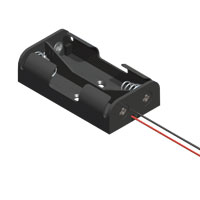
\includegraphics[scale=0.25]{pictures/2463-2469-2473.jpg}};
            \end{scope}
        }{
            \draw (0,0) rectangle (3,1.5) ;
        }{Amazon}{Porta Pilas} {3V} {1A} 
        
        \connectorinfo{Codigo}{2463}{
            \tabitem \textbf{Fabricante}: Keystone
        }
        & \multicolumn{4}{|l|}{\tabitem Modificado, terminado en un JST XH2.54 2 vias} \\
        \hline
        \connectorblockinfo{Uso}{Dcc Decoder Config - Portable}
        \connectorblockinfo{Ubicacion}{Terraza}
    \end{tabular}
    \caption{Porta Pilas 2463}
    \label{tab:pp2463}
\end{table}